% !TeX spellcheck = hu_HU
% !TeX encoding = UTF-8
% !TeX program = xelatex

\documentclass[11pt,a4paper,oneside]{report}

% thanks to http://tex.stackexchange.com/a/47579/71109
\usepackage{ifxetex}
\usepackage{ifluatex}
\newif\ifxetexorluatex % a new conditional starts as false
\ifnum 0\ifxetex 1\fi\ifluatex 1\fi>0
   \xetexorluatextrue
\fi

\ifxetexorluatex
  \usepackage{fontspec}
\else
  \usepackage[T1]{fontenc}
  \usepackage[utf8]{inputenc}
  \usepackage[lighttt]{lmodern}
\fi

\usepackage[english,magyar]{babel} % Alapértelmezés szerint utoljára definiált nyelv lesz aktív, de később külön beállítjuk az aktív nyelvet.

%\usepackage{cmap}
\usepackage{amsfonts,amsmath,amssymb} % Mathematical symbols.
%\usepackage[ruled,boxed,resetcount,linesnumbered]{algorithm2e} % For pseudocodes. % beware: this is not compatible with LuaLaTeX, see http://tex.stackexchange.com/questions/34814/lualatex-and-algorithm2e
\usepackage{booktabs} % For publication quality tables for LaTeX
\usepackage{graphicx}

%\usepackage{fancyhdr}
%\usepackage{lastpage}

\usepackage{anysize}
%\usepackage{sectsty}
\usepackage{setspace} % For setting line spacing

\usepackage[unicode]{hyperref} % For hyperlinks in the generated document.
\usepackage{xcolor}
\usepackage{listings} % For source code snippets.

\usepackage[amsmath,thmmarks]{ntheorem} % Theorem-like environments.

\usepackage[hang]{caption}

\singlespacing

\newcommand{\selecthungarian}{
	\selectlanguage{magyar}
	\setlength{\parindent}{2em}
	\setlength{\parskip}{0em}
	\frenchspacing
}

\newcommand{\selectenglish}{
	\selectlanguage{english}
	\setlength{\parindent}{0em}
	\setlength{\parskip}{0.5em}
	\nonfrenchspacing
	\renewcommand{\figureautorefname}{Figure}
	\renewcommand{\tableautorefname}{Table}
	\renewcommand{\partautorefname}{Part}
	\renewcommand{\chapterautorefname}{Chapter}
	\renewcommand{\sectionautorefname}{Section}
	\renewcommand{\subsectionautorefname}{Section}
	\renewcommand{\subsubsectionautorefname}{Section}
}

\usepackage[numbers]{natbib}
\usepackage{xspace}
\usepackage{indentfirst}


\newcommand{\vikszerzoVezeteknev}{Kovács}
\newcommand{\vikszerzoKeresztnev}{Bálint}

\newcommand{\vikkonzulensAMegszolitas}{Dr.~}
\newcommand{\vikkonzulensAVezeteknev}{Simon}
\newcommand{\vikkonzulensAKeresztnev}{Balázs}

\newcommand{\vikkonzulensBMegszolitas}{}
\newcommand{\vikkonzulensBVezeteknev}{}
\newcommand{\vikkonzulensBKeresztnev}{}

\newcommand{\vikkonzulensCMegszolitas}{}
\newcommand{\vikkonzulensCVezeteknev}{}
\newcommand{\vikkonzulensCKeresztnev}{}

\newcommand{\vikcim}{Dokumentumok nyomtatását optimalizáló szoftver fejlesztése} % Cím
\newcommand{\viktanszek}{\bmeiit} % Tanszék
\newcommand{\vikdoktipus}{\bsconlab} % Dokumentum típusa (\bsc vagy \msc)

\newcommand{\szerzoMeta}{\vikszerzoVezeteknev{} \vikszerzoKeresztnev} % egy szerző esetén

%--------------------------------------------------------------------------------------
% Elnevezések
%--------------------------------------------------------------------------------------
\newcommand{\bme}{Budapesti Műszaki és Gazdaságtudományi Egyetem}
\newcommand{\vik}{Villamosmérnöki és Informatikai Kar}

\newcommand{\bmeiit}{Irányítástechnika és Informatika Tanszék}

\newcommand{\keszitette}{Készítette}
\newcommand{\konzulens}{Konzulens}

\newcommand{\bsc}{Szakdolgozat}
\newcommand{\msc}{Diplomaterv}
\newcommand{\tdk}{TDK dolgozat}
\newcommand{\bsconlab}{BSc Önálló laboratórium}
\newcommand{\msconlabi}{MSc Önálló laboratórium 1.}
\newcommand{\msconlabii}{MSc Önálló laboratórium 2.}

\newcommand{\pelda}{Példa}
\newcommand{\definicio}{Definíció}
\newcommand{\tetel}{Tétel}

\newcommand{\bevezetes}{Bevezetés}
\newcommand{\koszonetnyilvanitas}{Köszönetnyilvánítás}
\newcommand{\fuggelek}{Függelék}

% Opcionálisan átnevezhető címek
%\addto\captionsmagyar{%
%\renewcommand{\listfigurename}{Saját ábrajegyzék cím}
%\renewcommand{\listtablename}{Saját táblázatjegyzék cím}
%\renewcommand{\bibname}{Saját irodalomjegyzék név}
%}

\newcommand{\szerzo}{\vikszerzoVezeteknev{} \vikszerzoKeresztnev}
\newcommand{\vikkonzulensA}{\vikkonzulensAMegszolitas\vikkonzulensAVezeteknev{} \vikkonzulensAKeresztnev}
\newcommand{\vikkonzulensB}{\vikkonzulensBMegszolitas\vikkonzulensBVezeteknev{} \vikkonzulensBKeresztnev}
\newcommand{\vikkonzulensC}{\vikkonzulensCMegszolitas\vikkonzulensCVezeteknev{} \vikkonzulensCKeresztnev}

\newcommand{\selectthesislanguage}{\selecthungarian}

\bibliographystyle{huplain}

\def\lstlistingname{lista}

\newcommand{\appendixnumber}{6}  % a fofejezet-szamlalo az angol ABC 6. betuje (F) lesz


%--------------------------------------------------------------------------------------
% Page layout setup
%--------------------------------------------------------------------------------------
% we need to redefine the pagestyle plain
% another possibility is to use the body of this command without \fancypagestyle
% and use \pagestyle{fancy} but in that case the special pages
% (like the ToC, the References, and the Chapter pages)remain in plane style

\pagestyle{plain}
% TODO: don't forget to change for binding
\marginsize{30mm}{30mm}{15mm}{15mm}

\setcounter{tocdepth}{3}
%\sectionfont{\large\upshape\bfseries}
\setcounter{secnumdepth}{3}

\sloppy % Margón túllógó sorok tiltása.
\widowpenalty=10000 \clubpenalty=10000 %A fattyú- és árvasorok elkerülése
\def\hyph{-\penalty0\hskip0pt\relax} % Kötőjeles szavak elválasztásának engedélyezése


%--------------------------------------------------------------------------------------
% Setup hyperref package
%--------------------------------------------------------------------------------------
\hypersetup{
    % bookmarks=true,            % show bookmarks bar?
    unicode=true,              % non-Latin characters in Acrobat's bookmarks
    pdftitle={\vikcim},        % title
    pdfauthor={\szerzoMeta},    % author
    pdfsubject={\vikdoktipus}, % subject of the document
    pdfcreator={\szerzoMeta},   % creator of the document
    pdfproducer={},    % producer of the document
    pdfkeywords={},    % list of keywords (separate then by comma)
    pdfnewwindow=true,         % links in new window
    colorlinks=true,           % false: boxed links; true: colored links
    linkcolor=black,           % color of internal links
    citecolor=black,           % color of links to bibliography
    filecolor=black,           % color of file links
    urlcolor=black             % color of external links
}


%--------------------------------------------------------------------------------------
% Set up listings
%--------------------------------------------------------------------------------------
\definecolor{lightgray}{rgb}{0.95,0.95,0.95}
\lstset{
	basicstyle=\scriptsize\ttfamily, % print whole listing small
	keywordstyle=\color{black}\bfseries, % bold black keywords
	identifierstyle=, % nothing happens
	% default behavior: comments in italic, to change use
	% commentstyle=\color{green}, % for e.g. green comments
	stringstyle=\scriptsize,
	showstringspaces=false, % no special string spaces
	aboveskip=3pt,
	belowskip=3pt,
	backgroundcolor=\color{lightgray},
	columns=flexible,
	keepspaces=true,
	escapeinside={(*@}{@*)},
	captionpos=b,
	breaklines=true,
	frame=single,
	float=!ht,
	tabsize=2,
	literate=*
		{á}{{\'a}}1	{é}{{\'e}}1	{í}{{\'i}}1	{ó}{{\'o}}1	{ö}{{\"o}}1	{ő}{{\H{o}}}1	{ú}{{\'u}}1	{ü}{{\"u}}1	{ű}{{\H{u}}}1
		{Á}{{\'A}}1	{É}{{\'E}}1	{Í}{{\'I}}1	{Ó}{{\'O}}1	{Ö}{{\"O}}1	{Ő}{{\H{O}}}1	{Ú}{{\'U}}1	{Ü}{{\"U}}1	{Ű}{{\H{U}}}1
}


%--------------------------------------------------------------------------------------
% Set up theorem-like environments
%--------------------------------------------------------------------------------------
% Using ntheorem package -- see http://www.math.washington.edu/tex-archive/macros/latex/contrib/ntheorem/ntheorem.pdf

\theoremstyle{plain}
\theoremseparator{.}
\newtheorem{example}{\pelda}

\theoremseparator{.}
%\theoremprework{\bigskip\hrule\medskip}
%\theorempostwork{\hrule\bigskip}
\theorembodyfont{\upshape}
\theoremsymbol{{\large \ensuremath{\centerdot}}}
\newtheorem{definition}{\definicio}

\theoremseparator{.}
%\theoremprework{\bigskip\hrule\medskip}
%\theorempostwork{\hrule\bigskip}
\newtheorem{theorem}{\tetel}


%--------------------------------------------------------------------------------------
% Some new commands and declarations
%--------------------------------------------------------------------------------------
\newcommand{\code}[1]{{\upshape\ttfamily\scriptsize\indent #1}}
\newcommand{\doi}[1]{DOI: \href{http://dx.doi.org/\detokenize{#1}}{\raggedright{\texttt{\detokenize{#1}}}}} % A hivatkozások közt így könnyebb DOI-t megadni.

\DeclareMathOperator*{\argmax}{arg\,max}
%\DeclareMathOperator*[1]{\floor}{arg\,max}
\DeclareMathOperator{\sign}{sgn}
\DeclareMathOperator{\rot}{rot}


%--------------------------------------------------------------------------------------
% Setup captions
%--------------------------------------------------------------------------------------
\captionsetup[figure]{
	width=.75\textwidth,
	aboveskip=10pt}

\renewcommand{\captionlabelfont}{\bf}
%\renewcommand{\captionfont}{\footnotesize\it}

%--------------------------------------------------------------------------------------
% Hyphenation exceptions
%--------------------------------------------------------------------------------------
\hyphenation{Shakes-peare Mar-seilles ár-víz-tű-rő tü-kör-fú-ró-gép}


\author{\vikszerzo}
\title{\viktitle}



\begin{document}

\pagenumbering{gobble}

\selectthesislanguage

\hypersetup{pageanchor=false}
%--------------------------------------------------------------------------------------
%	The title page
%--------------------------------------------------------------------------------------
\begin{titlepage}
\begin{center}

\includegraphics[width=60mm,keepaspectratio]{figures/bme_logo.pdf}\\
\vspace{0.3cm}
\textbf{\bme}\\
\textmd{\vik}\\
\textmd{\viktanszek}\\[5cm]

\vspace{0.4cm}
{\huge \bfseries \vikcim}\\[0.8cm]
\vspace{0.5cm}
\textsc{\Large \vikdoktipus}\\[4cm]

{
	\renewcommand{\arraystretch}{0.85}
	\begin{tabular}{cc}
	 \makebox[7cm]{\emph{\keszitette}} & \makebox[7cm]{\emph{\konzulens}} \\ \noalign{\smallskip}
	 \makebox[7cm]{\szerzo} & \makebox[7cm]{\vikkonzulensA} \\
	  & \makebox[7cm]{\vikkonzulensB} \\
	  & \makebox[7cm]{\vikkonzulensC} \\
	\end{tabular}
}

\vfill
{\large \today}
\end{center}
\end{titlepage}
\hypersetup{pageanchor=false}



\tableofcontents\vfill

\pagenumbering{arabic}

%TODO import your own content
\chapter{\bevezetes}

Nagyjából egy évvel ezelőtt csatlakoztam a KBPR kollégiumi öntevékeny körbe. A kör végzi el a kollégium szinte minden nyomtatási munkáját különböző partnerek nyomtatóin, többek közt egy Canon imagePROGRAF PRO-4600 plotteren. Papírtekercsekre nyomtatunk, viszont a kinyomtatott dokumentumok nem mindig tekercs szélességűek. Ez kimondottan gyakori eset, hiszen a legtöbb esetben A4-es méretben nyomtatunk, csak vastagabb, minőségibb papírra. Ilyen esetekre szolgált egy \href{fig:old_ui}{Adobe Photoshop script}, ami megpróbálta úgy elrendezni a megadott dokumentumokat, hogy azok egy tekercs szélességű rácson a lehető legkevesebb papírfelesleggel helyezkedjenek el, majd hozzáadott segédvonalakat, amik mentén később a kívánt méretre lehet vágni a kinyomtatott papírt.

Ez a script több hallgató keze műve volt, más-más verziói különböző funkcionalitást voltak képtelenek megvalósítani. Több sebből vérzett, de a legkevésbé sem tudom emiatt az eredeti szerzőit hibáztatni - a scriptet egy évvel ezelőtt erőteljesen refaktoráltam, és saját magam is szembesültem az Adobe ExtendScript nehézségeivel. A projekt nyílt forráskódú és a \href{https://github.com/SCH-KB-PR/kbpr-ps}{https://github.com/SCH-KB-PR/kbpr-ps} oldalon érhető el.

Felmerült az is, hogy keressünk már létező, erre specializálódó szoftvert. Egy plottercsere után erre sor is került, ugyanis járt mellé több különböző hivatalos Canon szoftver, azonban egyikük sem felelt meg a céljainknak, hasonlóképp mindegyikből hiányzott egy-egy funkció, amire szükségünk volt, nem beszélve arról, hogy hasonlóképp lassúak és nehezen használhatóak voltak, és hogy kizárólag Windows operációs rendszer alatt működnek.

A refaktorált script egy nagy erőlelépést jelentett, és gyorsan áttértünk a használatára. Azonban ez sem volt tökéletes, főként a Photoshop hatalmas overheadje miatt: a dokumentumok generálása sokáig tartott, és volt, hogy a rendelkezésre álló 8 GB ram sem volt elég. Ezeket a program script jellegéből adódóan nem volt lehetőségem tovább optimalizálni, ezért is szerettem volna elkészíteni egy hasonló programot, ami már a kezdetektől fogva törekszik az optimalizációra. Felmerült továbbá az az ötlet is, hogy tudjunk különböző méretű képeket egyszerre nyomtatni, erre még később kitérek.

Az ötlet még 2024 végén érkezett, amikor egy közös szoftverfejlesztési projektet szerettünk volna egy barátommal, Orbán Levente Lászlóval. Eleinte nem volt szilárd elképzelésünk, viszont annyi biztos volt, hogy nyílt forráskódú és elsősorban Linux operációs rendszert támogató programot szeretnénk közösen készíteni, ahol a nyelvi elemek terén ő tudna engem, a tervezés terén pedig én tudnám őt mentorálni. Az ő hozzájárulásával választottam az akkor még felettébb kezdetleges projektet az önálló laboratóriumom témájának, és a munkáját részletezni fogom.

\break

A továbbiakban szeretnék részletesebben kitérni a program specifikációjára, a rendszer tervére, annak megvalósítására és a felmerült nehézségekre, majd a szoftver tesztelésre, értékelésére, végül a projekt jövőjére. Mellékletként egy rövid felhasználói kézikönyvet is készítettem.

\begin{figure}[h]
    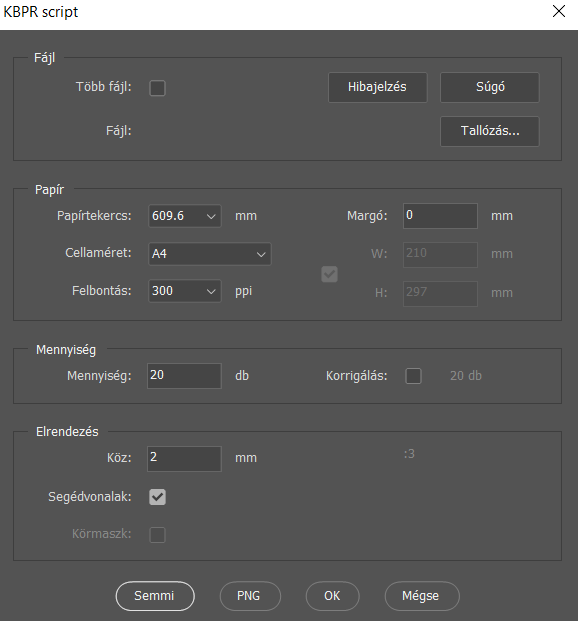
\includegraphics[width=\textwidth]{figures/script_showcase.png}
    \label{fig:old_ui}
    \caption{A kör által Photoshop script felhasználói felülete}
\end{figure}
\chapter{Specifikáció}

A feladatom tehát egy dokumentumok nyomtatását optimalizáló szoftver volt, ami minimalizálja az elrendezésből adódó papírfelesleget, ügyelve a program teljesítményére és annak könnyen használhatóságára.

\section{Funkcionális követelmények}
\begin{itemize}
    \item A rendszer legyen képes egy tekercs szélességű dokumentum elkészítésében.
    \item A dokumentumon a kívánt mennyiségben szerepeljen(ek) a megadott kép(ek).
    \item A képek a kívánt fizikai méretben szerepeljenek.
    \item A program legyen képes különböző pixelsűrűségeket (mn. dpi/ppi) kezelni.
    \item A képek fizikai mérete lehessen előre megadott szabvány méretű (pl. A4).
    \item A tekercsek fizikai mérete lehessen előre megadott szélességű.
    \item A képek közé lehessen állítható méretű térközt rakni.
    \item A dokumentum széleire lehessen állítható méretű margót tenni.
    \item A dokumentum lehessen vágóasztallal (széltől szélig) vágható.
    \item Legyen a képek vágását segítő segédvonal, ami mentén a dokumentum vágóasztallal vágható.
    \item A dokumentum lehessen nyomtatható és/vagy lehessen képi formátumban exportálni.
\end{itemize}

\section{Nem funkcionális követelmények}
\begin{itemize}
    \item A program törekedjem a gyors dokumentumgenerálásra. 
    \item A programhoz tartozzon egy grafikus felhasználói felület.
    \item A felhasználói felület legyen intuitív.
    \item A program törekedjen az effektív memóriahasználatra.
    \item A program működjön Linux operációs rendszer alatt (is).
    \item A program legyen befogadóképes a jövőbeli új funkciókra.
\end{itemize}
\chapter{Tervezés}

A tervezéshet a mellékelt UML diagramokat készítettem. A megvalósítás nagyjából követi ezt az architektúrát, pár apróbb eltéréssel és kiegészítéssel.

A projekt a printf nevet kapta.

\section{Kép betöltés, konfigurálás}

A bemeneti képeket tartalmazó és manipuláló osztályok tervezésénél különösen nagy hangsúlyt helyeztem a teljesítményre. Az \href{fig:ImageSource_uml}{ábrán} látszik, hogy a forrásfájlokat pixelenként tároljuk, és számontartjuk a hozzájuk tartozó filtereket. A filterek tudják transzformálni és manipulálni a képet (pl. méret, forgatás, maszk, segédvonalak). Az eredeti képet mindig megőrizzük, hogy a filterek ne legyenek destruktívak. Annak érdekében, hogy a filtereket ne kelljen minden egyes elérésnél újraszámolni vezettem be egy cachet. Ha változnak a filterek, a cache piszkos lesz, és a következő elérésnél újraszámolódik.

\section{Képgenerálás, algoritmusok}

A képgenerálás folyamata elsőre talán triviális. Helyezzünk el a képeinket egy rácson, aszerint elforgatva, hogy hogyan keletkezik kevesebb felesleg, figyelembe véve a margót és a térközt. A régi scriptünk is ezt az algoritmust követte, és az eredménye is megfelel az elvárásainknak. Ez mindaddig működik, amíg a forrásfájljaink méretei megegyeznek. Ha már több, különböző méretű képet kell minimális feleslegre, azaz minimális magasságú dokumentumra elhelyeznünk. Ez a probléma a ládapakolásra vezethető vissza, annak egy két dimenziós speciális esete, ahol figyelembe kell vegyük azt, hogy az eredményt vágóasztallal vágni tudjuk. Ez azt jelenti hogy a dokumentumot valahol az egyik szélétől a szemközti széléig elvágva keletkezett részek vagy egy kép, vagy egy vágóasztallal tovább vágható csík.\footnote{\href{https://en.wikipedia.org/wiki/Guillotine_cutting}{Guillotine cutting - Wikipedia}} A ládapakolás problémája viszont egy NP nehéz probléma.\footnote{\href{https://en.wikipedia.org/wiki/Bin_packing_problem}{Bin packing problem - Wikipedia}} Orbán Levente talált egy tanulmányt\footnote{\href{https://sci-hub.se/10.1016/j.ipl.2015.08.008}{A priority heuristic for the guillotine rectangular packing problem}} ennek kapcsán, ami ugyan nem mindig optimális, de az igényeinknek megfelelő polinomiális algoriutmust tartalmaz. Az algoritmusból továbbá hiányzott az is, a keletkező felesleget töltse ki oda esetleg beférő képekkel.

Ennek fényében úgy döntöttünk, hogy támogassuk mindkét megközelítést, és majd a felhasználó dönt a különböző algoritmusok között. Erre a célra szolgál egy Tiling interface, ami megkapja a képek listáját és a dokumentum tulajdonságait.

\section{A felhasználói felület}

A legnagyobb szabadságunk a felhasználói felület kapcsán volt. Mindenképpen szerettem volna egy előnézetet, hogy még mentés előtt a felhasználó lássa az eredményt, és azt esetleg javítani tudja a bemenetek újrakonfigurálásával. A kezelés lépéseinek sorrendje alapján igyekeztem kialakítani a felület többi részét. Vannak bemeneti képeink, azokat szeretnénk egyesíteni, majd kinyomtatni. Képek, egyben, nyomtatás. Ezt balról jobbra elrendezve kapjuk meg a felület végleges tervét: balra a bemenetek, azok beállításai, középen egy előnézet, jobbra pedig a kimenet (generált dokumentum) beállításai, a generálás és az exportálás/nyomtatás gomb. A UI feladata lenne továbbá az előbeállítások betöltése és a filterek beállítása is. A bemenetek alapján meghívódik a generálás, ami elkészíti nekünk a kívánt képet, ezt fogjuk látni az előnézeten.

Az említett előbeállítások valamilyen fájlból betölthető konfigurációk, melyek vonatkozhatnak a bemenő képekre, a kimenő dokumentumra, valamint esetlegesen a nyomtatóra. Ezzel megoldható, hogy ne kelljen fejben tartanunk a tekercsek és a papírok szabványainak méretét.


\begin{figure}
    \centering
    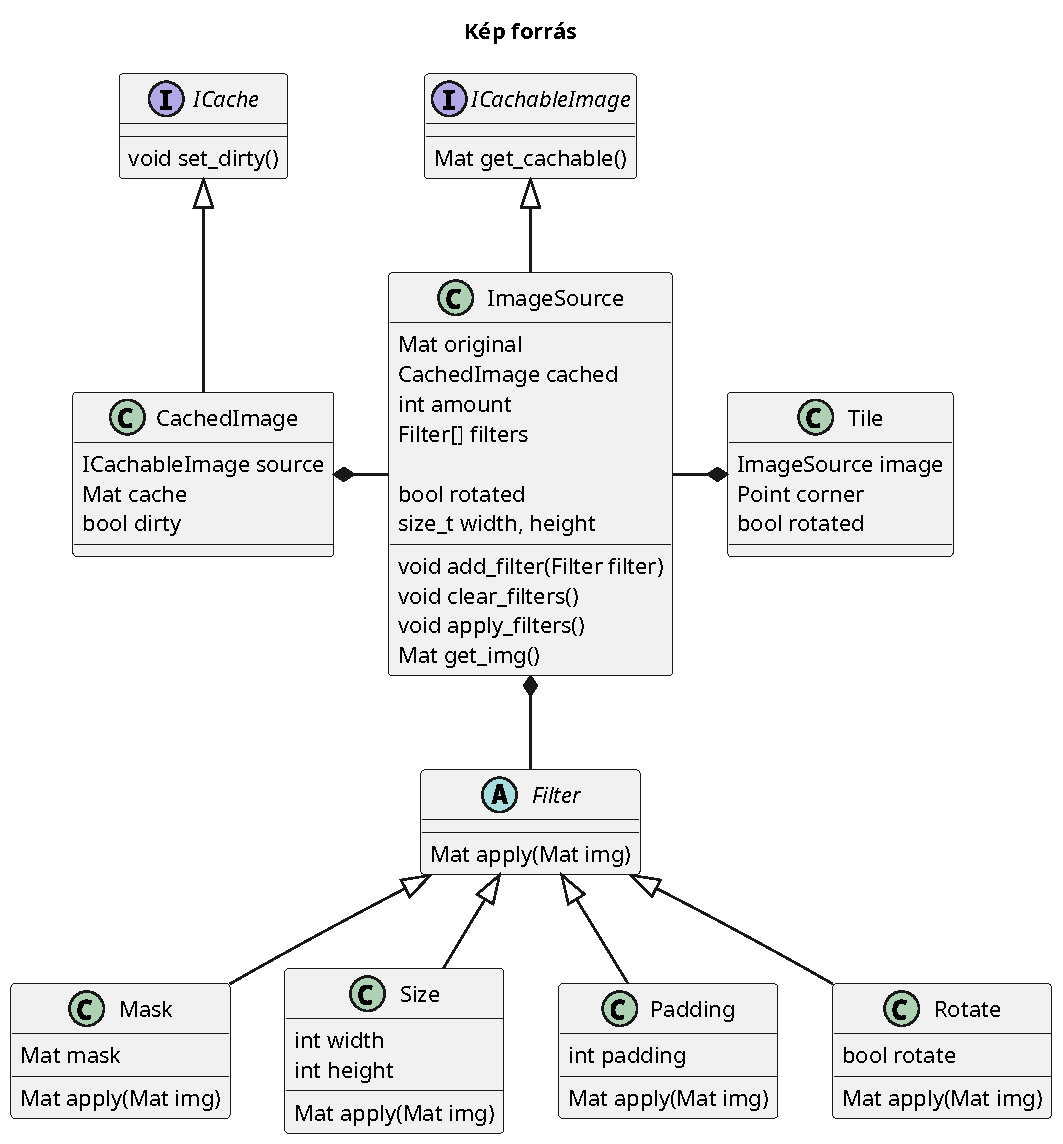
\includegraphics[width=15cm]{figures/uml/img_source.pdf}
    \label{fig:ImageSource_uml}
\end{figure}

\begin{figure}
    \centering
    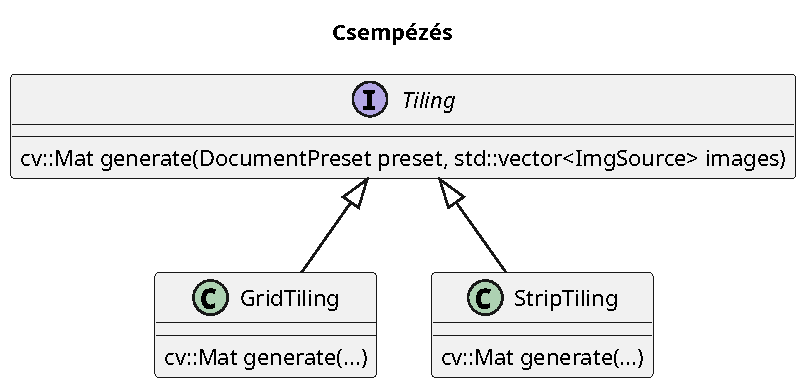
\includegraphics[width=12cm]{figures/uml/tiling.pdf}
    \label{fig:Tiling_uml}
\end{figure}

\begin{figure}
    \centering
    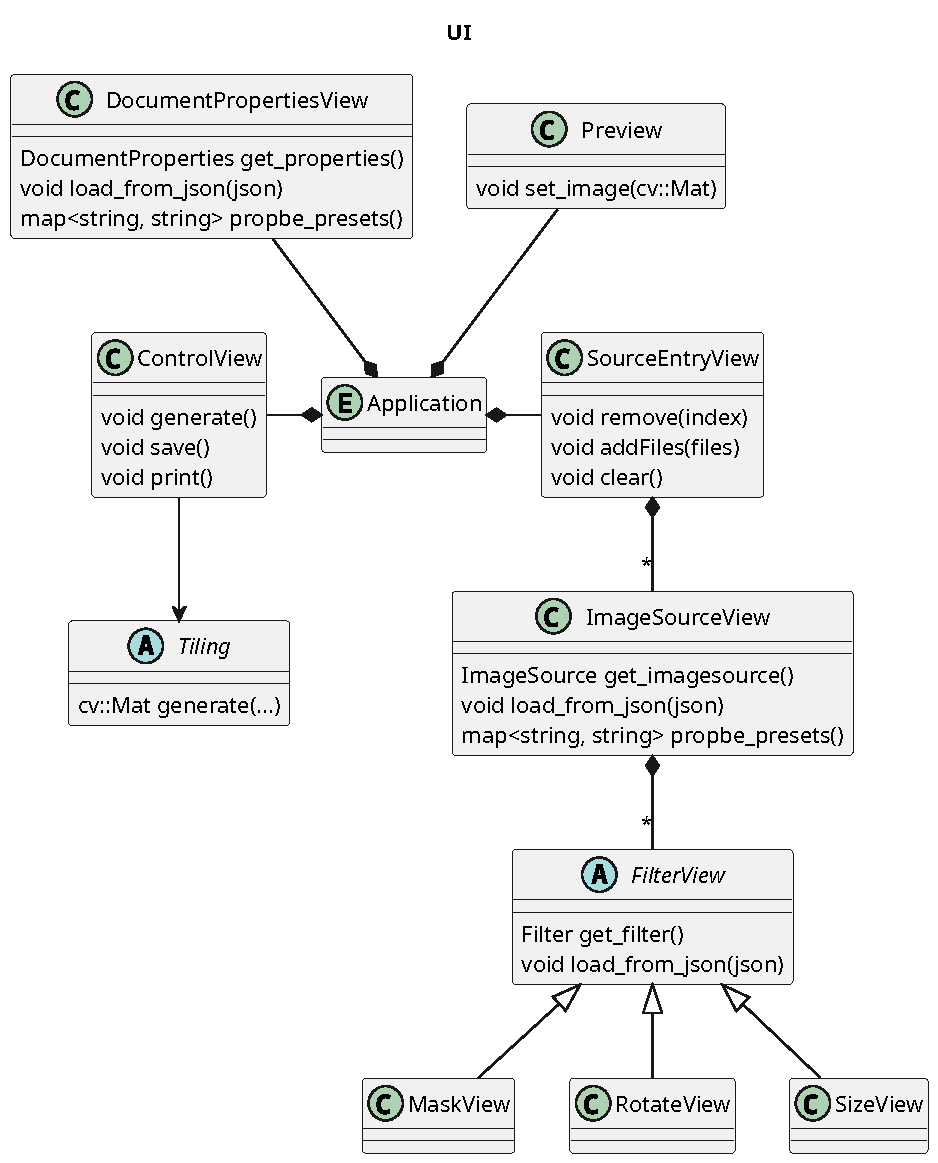
\includegraphics[width=14cm]{figures/uml/ui.pdf}
    \label{fig:UI_uml}
\end{figure}

\chapter{Megvalósítás}

\section{Technológiák}

A felhasznált technológiákat a projekt fókuszai alapján választottuk ki. 
A választásunk a C++-ra esett, annak példátlan sebességéből, és a memória kezelését illető sajátosságaiból. Beépített könyvtára képmanipulációra viszont nincsen, ehhez az \href{https://en.wikipedia.org/wiki/OpenCV}{OpenCV} könyvtárat választottuk, annak nyílt forráskódja és optimalizáltsága miatt.
A felhasználói felülethez egy szintén platformfüggetlen megoldást szerettünk volna, ezért a \href{https://en.wikipedia.org/wiki/Qt_(software)}{Qt} melett döntöttünk. 

\section{Fejlesztést segítő eszközök}

A kooperációt a GitHubon terveztük lebonyolítani, és tervben voltak GitHub actionök az automatikus ellenőrzésekhez is. A program buildeléséhez több másik próbálkozás után a \href{https://en.wikipedia.org/wiki/Meson_(software)}{Meson}t választottuk. A tervezéshez szükséges diagramokhoz \href{https://en.wikipedia.org/wiki/PlantUML}{PlantUML}-t használtam, fejlesztői környezetnek pedig a \href{https://en.wikipedia.org/wiki/Visual_Studio_Code}{Visual Studio Code}-ot

\section{Fejlesztés és nehézségek}

\subsection{Buildelés}

A legelső nehézség már fejlesztés legelején szembe jött velünk: a buildelés. Egyikünknek sem volt sok tapasztalata a build rendszerekkel, ezért erre sok időnk elment. Külön kihívás volt, külső könyvtárakat is linkelnünk kellett, amiknek a további konfigurációja messze nem volt triviális. Eleinte a \href{https://en.wikipedia.org/wiki/CMake}{CMake}-kel és a \href{https://en.wikipedia.org/wiki/Vcpkg}{vcpkg}-vel próbálkoztunk, de nem sikerült működésre bírnunk. Egy barátom, Bánáti Benedek javaslatára kezdtük el használni a Mesont, ami sokkal barátságosabbnak bizonyult. A Meson használata során is ütköztem további problémákba, mert a Qt header fájlokat a fordítás előtt még fel kell dolgozni, és erre csak CMake-es példákat találtam.

Indokalatlanul sok időnk ment el rá, és Windowson azóta sem tudunk buildelni\footnote{nem lehetetlen, csak Windowson egy nagyságrenddel macerásabb előkészíteni a buildelési környezetet}, de ez sajnos a C++ velejárója.

\subsection{Modell és generálás}

A modell implementálása a tervek alapján gördülékenyen ment, és a régi módszerrel történő generálás prototípusa is hamar elkészült. A prototípus sebességével elégedett voltam, nagyságrendekkel gyorsabb volt, mint ugyanez Photoshopban. A strip tiling algoritmust megegyezés szerint Levi készítette volna, ennek az implementálására viszont nem került még sor, kollégám sűrű negyedik félévéből adódóan.

\subsection{A Qt és a felhasználói felület}

Ehhez a projekthez használtam először Qt-ot, ezért eleinte nagyon lassan haladt a felület fejlesztése. A Qt Quick használata mellett döntöttem, melynek segítségével egy deklaratív UI leíró nyelven (\href{https://en.wikipedia.org/wiki/QML}{QML}) lehet elkészíteni a felhasználó felületet. Néhány dologban hasonlít más UI leíró nyelvekre, nem kellett nulláról kezdenem, de azért még így is akadtak nehézségek bőven. Legfőképp a nézet és a modell összeköttetése volt az, amiben hamar elakadtam. Hogy egy osztályt elérnjünk QML-ből, ahhoz az osztályunknak nem elég a Qt osztályokból származnia, hanem még különféle makrókkal is el kell látnunk a tagváltozóinkat, a függvényeinket, és még az osztályainkait is. Ezen osztályok header fájljait fordítás előtt fel kell dolgoznunk a Qt MOC\footnote{Meta-Object Compiler}-ével, hogy az osztályaink elérhetőek legyenek QML-ből, és hogy ezekről futásidejű típusinformációink is legyenek. 

Túlságosan nem mennék részletekbe a UI implementációját illetően, csupán pár érdekesebb részét emelném ki. A lista, amin a bemenetek láthatóak lusta, azaz a nem látható elemeket és a hozzá tartozó állapotot és objektumokat a rendszer felszabadítja. Ezt az implementáció során figyelembe is vettem, és egy indirekcióval oldottam meg, arra viszont nem figyeltem, hogy a filterek modelljével való összeköttetés UI szinten valósult meg, és ez az összeköttetés csak addig van jelen, amíg az elem látható. Erre sajnos csak az éles tesztnél találtam rá, mert itt teszteltem először háromnál több képpel a programot. A hiba azóta javítva lett.

Egy másik érdekesség talán az előbeállítások betöltésének folyamata. A program JSON fájlokból olvas be, ezek létezését először az adott mappában felderíti, majd rögzíti a név-elérési út párokat. Betöltéskor a JSON-ben jelenlévő értékek felülírják az eddigi beállításainkat, a hiányzó kulcsokhoz tartozó értékekre pedig nem lesznek hatással. A beállítások a már említett módon elkülönülnek (papír, dokumentum, maszk), de tovább tudnak propagálni más részekre. Így lehetséges például az, hogy a nagyplakát papírbeállítás hatással van a tekercs szélességére, vagy a matrica beállítás a képpontsűrűségre. 

\subsection{Több szálon futás}

Ugyan ügyeltem, hogy minél gyorsabb legyen a kép generálása, ez a folyamat így is tud időigényes lenni. Itt ugyan csak pár másodpercről beszélünk, de ez elég arra, hogy a Qt felület azt higgye, hogy az alkalmazásunk lefagyott. Ez egy elég gyakori eset a szoftverfejlesztésben, már jól ismert megoldással: szervezzük át külön szálra, hogy ne a fő szálon történjen a generálás. Az implementáció itt sem volt zökkenőmentes, hiszen valahogy jeleznünk is kell a UI felé, hogy frissült az eredmény, de vannak erre ún. signalok a Qt-ban. Hasonló problémába ütköztem a kép elmentésénél, ami még tovább tart, de ezt is ugyan úgy javítani tudtam. 

\subsection{Exportálás}

Miután már a többszálúságot megoldottam a kép elmentése elsőre nem kimondottan volt kihívás, mert volt rá beépített függvény. Teszteléskor viszont sajnos kibukott, hogy a nyomtatáshoz használt szoftverünk miatt szükség lenne bizonyos metaadatokra, elsősorban a képpontsűrűségre (dpi), erre viszont a beépített megoldások nem voltak képesek. Ezt először \href{https://en.wikipedia.org/wiki/Exif}{EXIF} metaadatokkal próbáltam megoldani, amit a legtöbb képnézegető meg is jelenít. Windowson viszont kicsit más a helyzet, az ottani fájl tulajdonságoknál és így a nyomtató szoftverében sem jelent meg az EXIF-ban beállított dpi. Megpróbáltam valami hasonlót \href{https://en.wikipedia.org/wiki/Extensible_Metadata_Platform}{XMP}-mal is, de hiába. Az egyetlen lehetőségem, ami maradt, az az, hogy a fájl formátum fejlécben tároljam el. Ez persze formátumonként eltér és más-más implementációk tartoznak hozzá, nem úgy, mint az EXIF-nál. A veszteségmentességéből adódóan a PNG formátum melett döntöttem. Bármennyire is élveztem elmerülni a képformátumok kodekjeinek működésében, nem hiszem hogy ennek a projektnek a kereteiben szeretnék saját PNG tömörítőt írni (nem is beszélve arról, hogy a megoldásom messze nem lenne optimális), ezért különböző könyvtárakkal próbáltam ezt megoldani. A végső megoldás a \href{https://libspng.org/}{libspng} C könyvtárat használja. Igyekeztem elkerülni, hogy másolat készüljön a képekről a lemezen vagy a memóriában, ezt sajnos nem sikerült teljes mértékben megoldani. 

\subsection{Refaktorálás}

A félév vége felé haladva elkezdtem refaktorálni a forráskódot. Elkezdtem használni a shared és unique pointereket, megelőzve ezzel a legvalószínűbb memóriaszivárgásokat. A kód nincs dokumentálva, de követi a clean code elveit. 

\begin{figure}[h]
    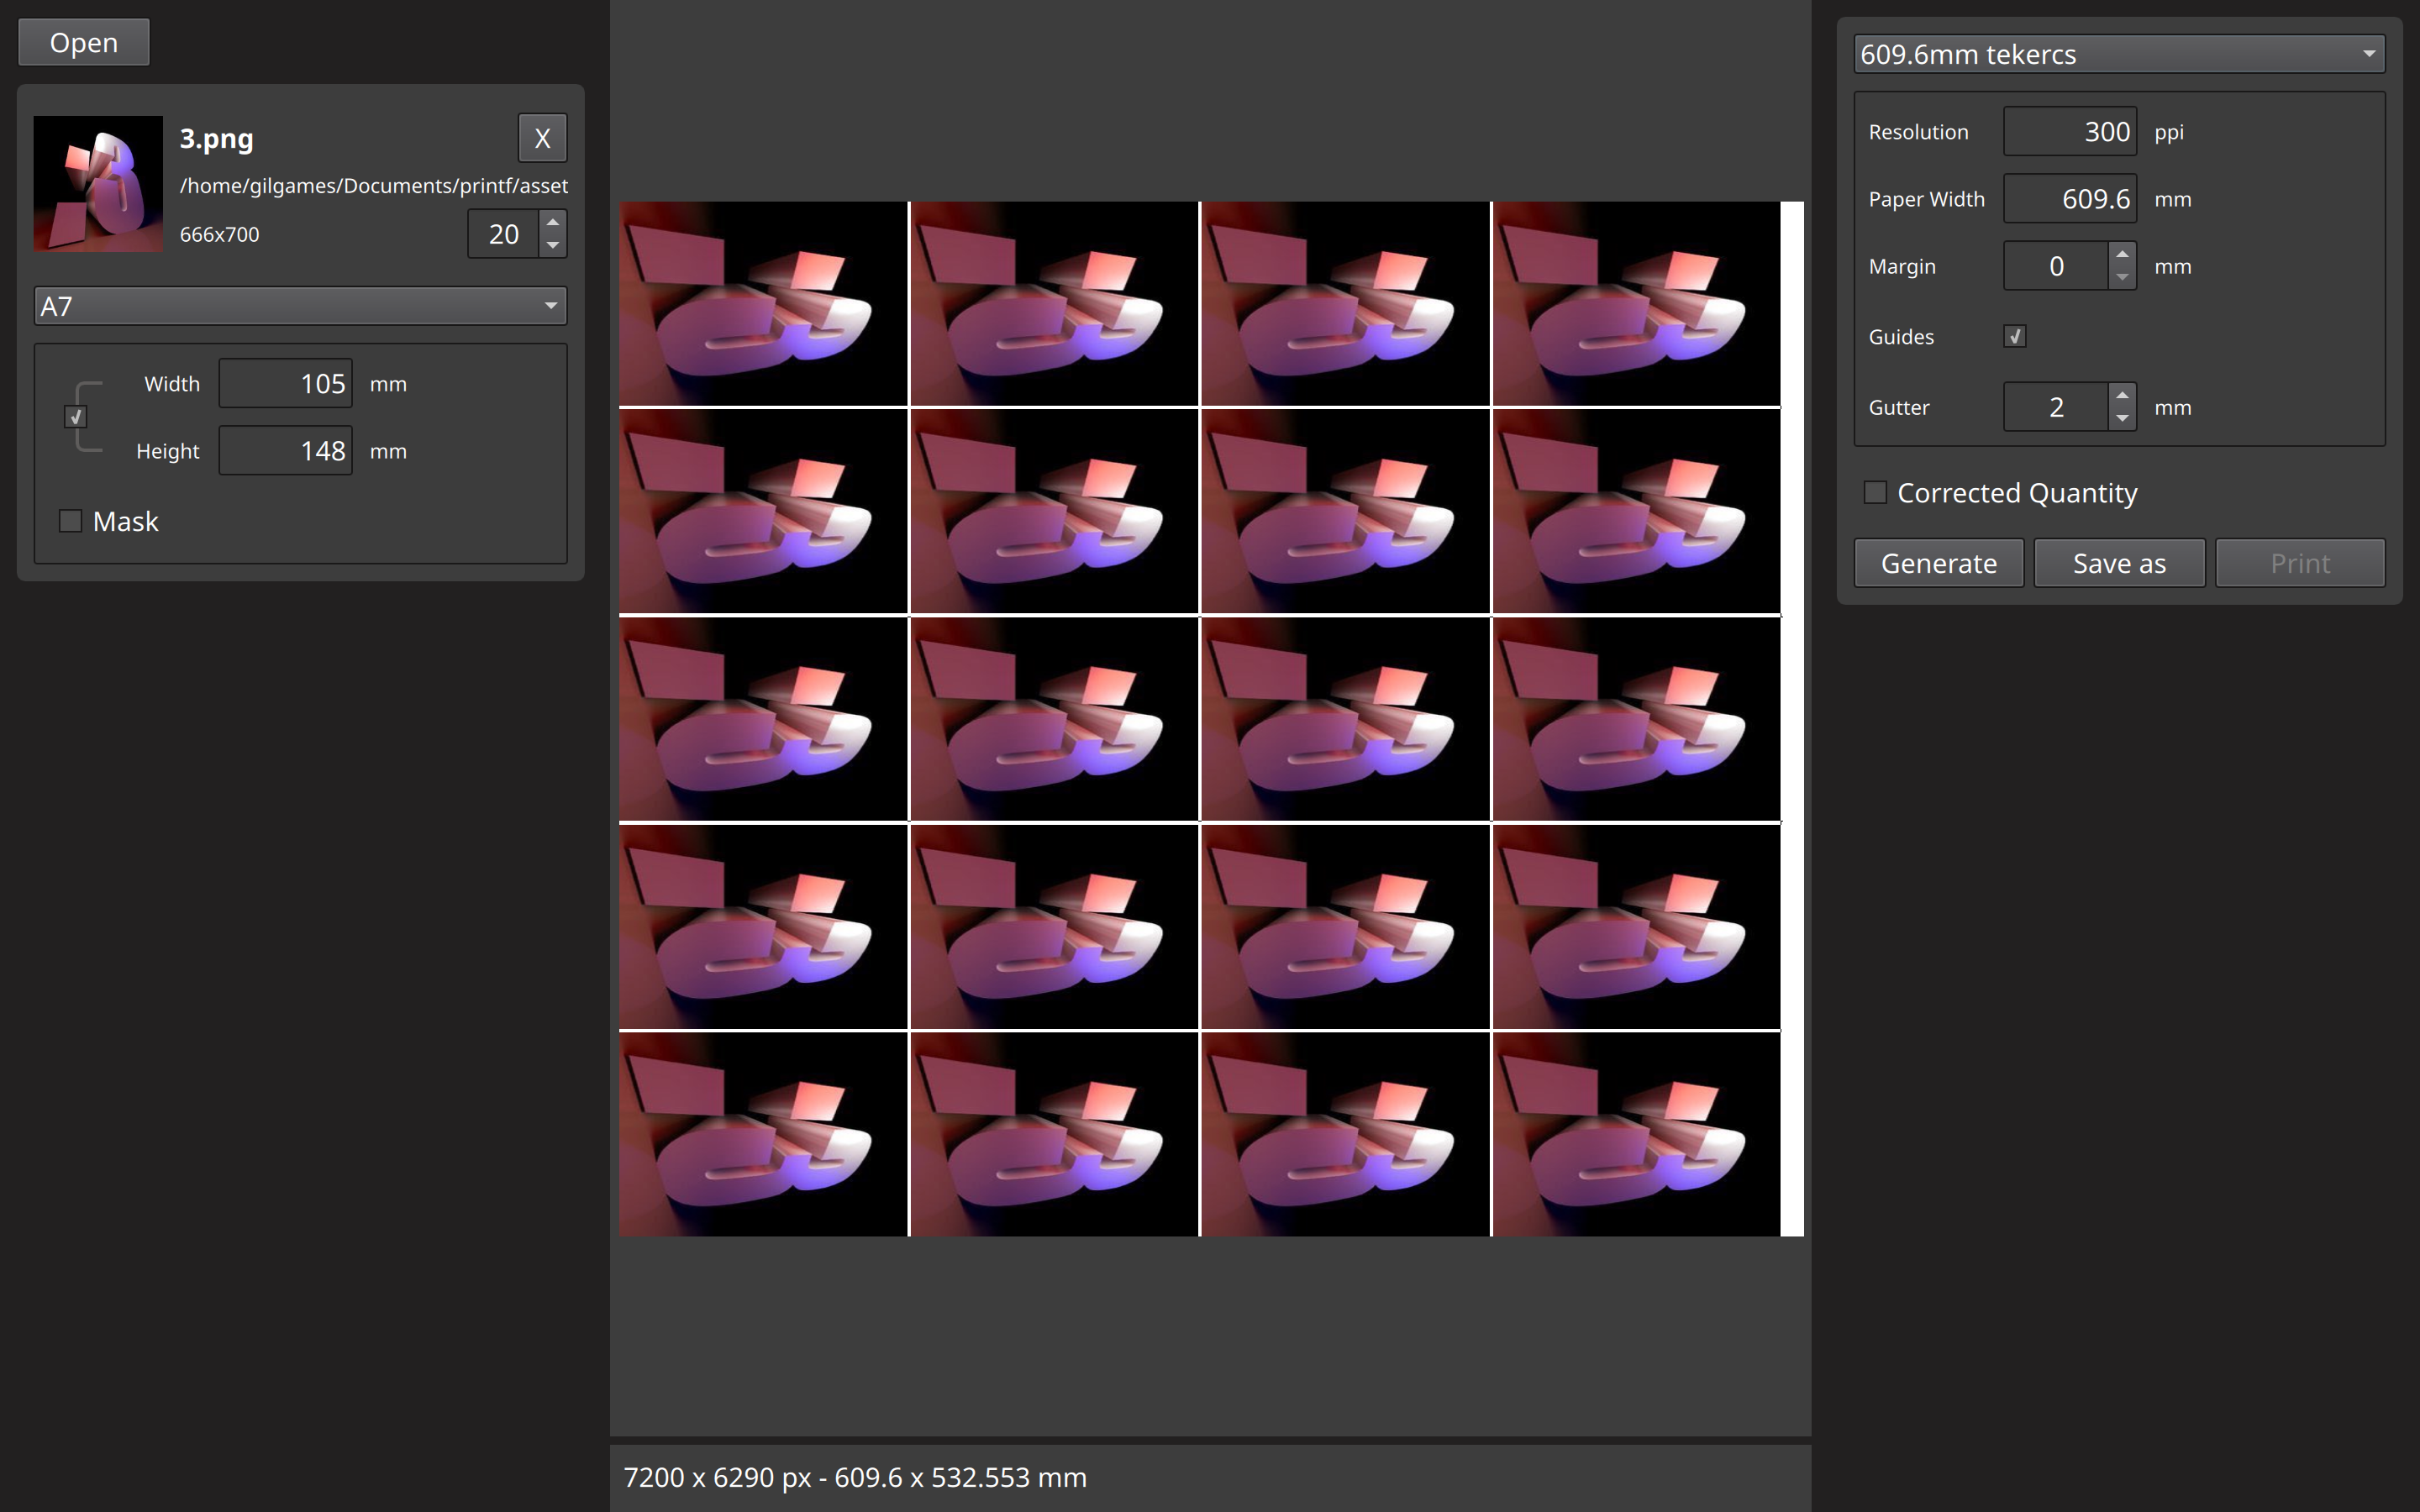
\includegraphics[width=\textwidth]{figures/ui_showcase.png}
    \caption{A felhasználói felület}
    \label{fig:ui_screenshot}
\end{figure}


%\label{page:last}
\end{document}
